\section*{Introduction}

Linear algebra is an excellent instrument for solving a wide variety of problems by utilizing matrices and vectors for data representation and analysis with the help of highly optimized routines. And whilst the matrices involved in a vast diversity of modern applications, e.g., recommender systems~\cite{amazon, gupta2020architectural} and graph analysis~\cite{graph1,graph2}, consist of a large number of elements, the major part of them are zeros. For example, the matrix representing YouTube's  social network connectivity contains only $2.31
\%$ non-zeros~\cite{leskovec2016snap}. Such a high sparsity incurs both computational and storage inefficiencies, requiring unnecessarily large storage occupied by zero elements and many operations on zeroes, where the result is obviously known beforehand. 
The traditional approach to address these inefficiencies is to compress the
matrix, store only the non-zero elements, and then operate only
on non-zero values.
Thus, the effect of matrices tending to be sparse in many applications makes the techniques of matrix compressed representation and sparse linear algebra to be an effective way of tackling problems in areas including but not limited to graph analysis~\cite{GAILLA}, computational biology~\cite{compBio} and machine learning~\cite{Kepner_2017}.

% Sparse linear algebra defines building blocks for expressing algorithms for already mentioned areas in a uniform way in terms of sparse matrix and vector operations over some semiring. Once such blocks are implemented in software (or hardware) according to, e.g., \emph{GraphBLAS}~\cite{buluc2017graphblas} standard, a myriad of expressible algorithms could be tuned and optimized at once by optimizing and tuning the building blocks. There are several implementations of GraphBLAS standard showing decent performance for both GPU~\cite{yang2020graphblast} and CPU~\cite{SuiteSparse} backends with one of them already speeding up graph database queries~\cite{redis}. However, typical CPUs and GPUs are proven to be underutilized~\cite{Florida,leskovec2016snap,Song_2016,zhang2020sparch}, i.e., their computing units do not achieve peak performance, for tasks that involve sparsity, due to being too general-purpose by design and suffering from the irregularity of memory accesses incurred by sparsity. 
\emph{GraphBLAS}~\cite{buluc2017graphblas} standard defines sparse linear algebra building blocks useful to express algorithms for already mentioned areas uniformly in terms of sparse matrix and vector operations over some semiring.
These include, for instance, matrix/vector multiplication, element-wise operations (e-wise for short), Kronecker product, masking, i.e., taking a subset of elements that satisfies the mask or its complement, etc.. These are sufficient to express a lot of algorithms, e.g. \emph{PageRank}, \emph{Breadth-First-Search}, \emph{Sparse Deep Neural Network}~\cite{SparseDNN}.


However, sparse computations appear to have a low arithmetic-to-me\-mo\-ry operations intensity, meaning that the main bottleneck of sparse algorithms is the sparse representation itself.
It induces pointer-chasing and presents irregularity of memory accesses.
Thus, a number of optimizations were identified~\cite{yang2020graphblast}, whose aim is to reduce the intensity of memory accesses, and the one considered in this work is \emph{fusion}.
Fusion simply stands for gluing several functions into one to remove intermediate data structures, namely those that are first constructed and then deconstructed.

An example of fusion could be seen in figure~\ref{fig:mask_fus}.
There a masked sparse matrix-spare vector multiplication (shown with $\otimes$) is depicted.
The mask simply takes the subset of the result, but fusing the mask inside the multiplication reduces the number of memory accesses by avoiding the construction of an intermediate matrix that would store the result of multiplication. 


\begin{figure}
    \centering
    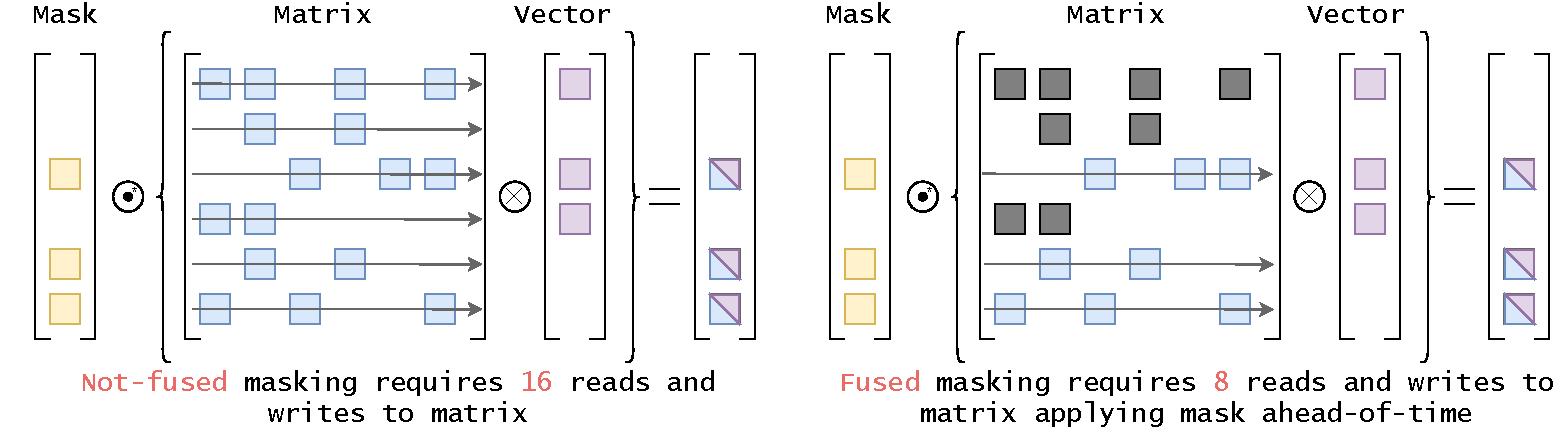
\includegraphics[width=\linewidth]{figures/MaskFusion.pdf}
    \caption{Mask fusion}
    \label{fig:mask_fus}
\end{figure}


In the case of loop-based programming, fusion simply stands for joining several loops into one to increase memory locality and reduce the number of required iterations.
It is a crucial technique in dense applications and is usually implemented as a part of affine transformations and polyhedral analysis~\cite{affine}. However, indexing in sparse applications is not an affine one.

% by a stage of \emph{polyhedral analysis}.
% This is extensively exploited in frameworks like TensorFlow and its XLA compiler~\cite{TensorFlowXLA}, where fusion is used to merge several GPU kernels into one to reduce both memory transfer and kernel start overheads. 

Some general-purpose solutions exist that support fusion (e.g., \cite{Futhark}) which are based on map/reduce semantics.
But in order to support sparse operations, they should be able to fuse across index arithmetic, which is not the case.
Also, at the moment neither SuiteSparse~\cite{newsuitesparse}  nor GraphBlast~\cite{yang2020graphblast} have adopted automatic fusion in their implementations but address the issue, and these are widely used GraphBLAS implementations for CPU and GPU platforms, respectively.

%but do have ad hoc solutions.
% In this work, we propose an approach to support automatic fusion for such applications and outline the overall solution design as well as present some intermediate evaluations of the approach.

Further, there are several implementations of GraphBLAS standard that show decent performance for both GPU~\cite{yang2020graphblast} and CPU~\cite{SuiteSparse} backends, with one of them already speeding up graph database queries~\cite{redis}. However, typical CPUs and GPUs were proven to be underutilized~\cite{Florida,leskovec2016snap,Song_2016,zhang2020sparch}, i.e., their computing units do not achieve peak performance, for tasks that involve sparsity, due to being too general-purpose by design and suffering from the irregularity of memory accesses incurred by sparsity. 

The traditional approach for problems when existing hardware does not provide enough performance or appear to be energy-inefficient for a particular application is the design of an application-specific processor. Such an approach has found a successful application in image processing~\cite{halide,redgrave2018pixel}, programmable networks~\cite{barefoot}, and machine learning~\cite{GoogleTPU,TensorFlowXLA}. Thus, a possible way of addressing the underutilization issues of the current hardware running sparse algorithms is the design of an application-specific processor that could handle sparse operations more efficiently. 

% Many modern application-specific processors come along with application-specific \emph{software}~\cite{TensorFlowXLA,halide}, i.e., domain-specific language, and a corresponding compiler, hence, the design of such a sparse system should both consider software and hardware parts.

And indeed, there are a number of works~\cite{Song_2016,SMASH,zhang2020sparch,Systolic} that implement specific hardware for sparse operations. 
However, they generally focus on sparse matrix-matrix and matrix-vector multiplications which are not enough to express a somewhat useful subset of sparse building blocks, i.e., blocks that appear to be useful to construct, e.g., some graph algorithms like finding maximal independent subset.
The low-level nature of such solutions makes it impossible to reason about them, which makes automatic fusion impossible. Finally,
% Hence, existing solutions do not consider a possibility of performing fusion and are too specialized. 
in such applications, the overall design energy consumption and performance are dominated by external memory accesses. Fusion reduces the number of such accesses and thus could improve the performance.


The traditional approach for developing hardware uses some low-level RTL programming, e.g., in SystemVerilog. However, high-level synthesis, a process when hardware is generated from a description given in a high-level language, makes reasoning about programs easier, opening opportunities for already mentioned fusion. Thus, the aim of this work is to compile sparse linear algebra programs into hardware with fusion optimization in mind. That will exploit the performance from the hardware side and amenability to optimizations from the software side.

% When used to create algorithms such blocks are often combined in a way that some optimizations become available. Given that, current solutions do not consider the software part of such systems, which should have enough expressive power and be amenable to certain optimizations, while implementing sparse matrix-matrix multiplication (or other blocks) entirely in hardware makes it impossible to perform specific optimizations~\cite{yang2020graphblast,fusion,KernelFusion}, that could increase the performance or reduce memory usage, and are easily expressible in terms of software. Notably, the works provide high-performance implementations of the components that constitute the execution pipeline of sparse algorithms, e.g., schedulers~\cite{zhang2020sparch}, sorters, communication units~\cite{Song_2016}, as well as hardware-effective storage and compression~\cite{SMASH}. Thus a promising approach could be in combining the best practices from hardware implementations and software optimizations finding the compromise between expressibility and performance

% The aim of this work is to co-design both hardware and software solution for acceleration of sparse linear algebra algorithms. This co-design addresses the issue of underutilization of CPUs and GPUs and the issue of inapplicability of certain optimizations in case of already designed sparse-specific processors. The work follows the experience of GraphBLAS implementations to specify the requirements for expected optimizations and expressivity power considering the software part of the system, and hardware primitives from~\cite{Song_2016,SMASH,zhang2020sparch,Systolic} to implement the hardware pipeline of sparse-specific units following dataflow HLS approach from~\cite{Edwards2019FHWP}.
